\documentclass[10pt, a4paper]{article}

%%%%%%%%%%%%%%
%  Packages  %
%%%%%%%%%%%%%%


\usepackage{page_format}
\usepackage{special}
\usepackage{hyperref}
\usepackage{tikz}
\usepackage[compat=1.1.0]{tikz-feynman}
\input{math_func}

\usepackage[sep=3pt,offset=0.5ex]{simpler-wick}
\newif\ifWickBelow
\WickBelowfalse
\pgfkeys{
  /simplerwick/below/.code={\WickBelowtrue},
}

\makeatletter
\def\swick@end#1#2{
  \swick@setfalse@#1
  \tikzexternaldisable
  \begin{tikzpicture}[remember picture, baseline=(swick-close#1.base)]
    \node[use as bounding box, inner sep=0pt, outer sep=0pt] (swick-close#1) {$\displaystyle #2$};
  \end{tikzpicture}
  \tikz[remember picture, overlay]
{
\ifWickBelow
    \draw ($(swick-open#1.south) + (0, -3pt)$) 
          -- ($(swick-open#1.base) + (0, -\swick@offset) + #1*(0, -\swick@sep)$) 
          -- ($(swick-close#1.base) + (0, -\swick@offset) + #1*(0, -\swick@sep)$) 
          -- ($(swick-close#1.south) + (0, -3pt)$);
\else
    \draw ($(swick-open#1.north) + (0, 3pt)$) 
          -- ($(swick-open#1.base) + (0, \swick@offset) + #1*(0, \swick@sep)$) 
          -- ($(swick-close#1.base) + (0, \swick@offset) + #1*(0, \swick@sep)$) 
          -- ($(swick-close#1.north) + (0, 3pt)$);
\fi}
\tikzexternalenable}
\makeatother

% References
\usepackage{biblatex}
\addbibresource{ref.bib}


%%%%%%%%%%%%
%  Colors  %
%%%%%%%%%%%%
% ! EDIT HERE !
\colorlet{chaptercolor}{red!70!black} % Foreground color.
\colorlet{chaptercolorback}{red!10!white} % Background color


%%%%%%%%%%%%%%
% Page titre %
%%%%%%%%%%%%%%
\title{Homework 2} % Title of the assignement.
\author{\PA} % Your name(s).
\teacher{Bindiya Arora and Dan Wohns} % Your teacher's name.
\class{Quantum Mechanics} % The class title.

\university{Perimeter Institute for Theoretical Physics} % University
\faculty{Perimeter Scholars International} % Faculty
%\departement{<Departement>} % Departement
\date{\today} % Date.


%%%%%%%%%%%%%%%%%%%%%%
% Begin the document %
%%%%%%%%%%%%%%%%%%%%%%
\begin{document}

% Make the title page.
\maketitlepage

% Make table of contents
\maketableofcontents

% Assignment starts here ----------------------------
\section{Two real scalars}

\begin{enumerate}
    \item[(a)] We are considering here perturbative results in the quantum field theory of two interacting real massive scalars $\varphi$, $\Phi$ with respective masses $m$ and $M$. The lagrangian density describing this theory is 
    \begin{align*}
        \mathcal{L} = \dfrac{1}{2}(\partial_\mu \varphi)^2 - \dfrac{1}{2} m^2 \varphi^2  + \dfrac{1}{2}(\partial_\mu \Phi)^2 - \dfrac{1}{2} M^2 \Phi^2 - \frac{g}{2! 1!} \Phi \varphi^2
    \end{align*}
    where $g$ descrives the coupling of the fields and is the parameter of our perturbative expansion. The position-space Feynman rules for perturbative computation of the interacting vacuum $\ket{\Omega}$ n-point functions $\bra{\Omega}T\varphi(x_1) \cdots \Phi(x_k) \cdots  \Phi(x_n)\ket{\Omega}$ for this theory are summed up graphically below:\\[0.3cm]
    \begin{minipage}{0.45\textwidth}
        \begin{center}
        \begin{tikzpicture}
            \begin{feynman}
              % Vertex with a label
              \vertex[label={[shift={(1cm, 0cm)}]right:$-ig \int \text{d}^4x$}] (v);
              \vertex[label={[shift={(0cm, 0.1cm)}]above:$x$}] (v);
              % External legs
              \vertex [left=of v] (a);
              \vertex [above right=of v] (b);
              \vertex [below right=of v] (c);
              \fill (v) circle (2pt);
              % Dashed line
              \diagram* {
                (a) -- [dashed] (v),
                (v) -- (b),
                (v) -- (c),
              };
            \end{feynman}
          \end{tikzpicture}
        \end{center}
    1. Every vertex in a diagram is associated to a four-position variable $x$. Its contribution to the symbolic representation of the amplitude is the integral $-ig \int \text{d}^4x$ acting on the propagators from the $x$ vertex to other vertices. \\[0.3cm]
    3. Divide the amplitude by the symmetry factor $S$ of the diagram. $S$ is computed graphically as the order of the fixed end-points automorphism group of the diagram.
    \end{minipage}%
    \hspace{0.3cm}
    \begin{minipage}{0.45\textwidth}
        \begin{center}
        \begin{tikzpicture}
            \begin{feynman}
                % Vertex with a label
                \vertex[label={[left=of v]:$x$}];
                \vertex[label={[shift={(0cm, 0cm)}]right:$y$}];
                \vertex[label={[shift={(-0.8cm, 0.1cm)}]above:$\Delta_{F}^{M}(x-y)$}];
                \vertex[label={[shift={(-0.8cm, -0.9cm)}]above:$1$}];
                % External legs
                \vertex [left=of v] (a);
                \vertex [below=1cm of v] (c); 
                \vertex [below=1cm of a, label={left:$x_1$}] (d); % Adjust the vertical position here

                \fill (a) circle (2pt);
                \fill (v) circle (2pt);
                \fill (d) circle (2pt);

        
                % Dashed line
                \diagram* {
                  (a) -- [dashed] (v),
                  (c) -- [dashed] (d),
                };
              \end{feynman}
          \end{tikzpicture}
        \begin{tikzpicture}
            \begin{feynman}
                % Vertex with a label
                \vertex[label={[left=of v]:$x$}];
                \vertex[label={[shift={(0cm, 0cm)}]right:$y$}];
                \vertex[label={[shift={(-0.8cm, 0.1cm)}]above:$\Delta_{F}^{m}(x-y)$}];
                \vertex[label={[shift={(-0.8cm, -0.9cm)}]above:$1$}];
                % External legs
                \vertex [left=of v] (a);
                \vertex [below=1cm of v] (c); 
                \vertex [below=1cm of a, label={left:$x_1$}] (d); % Adjust the vertical position here

                \fill (a) circle (2pt);
                \fill (v) circle (2pt);
                \fill (d) circle (2pt);

        
                % Dashed line
                \diagram* {
                  (a) -- (v),
                  (c) -- (d),
                };
              \end{feynman}
          \end{tikzpicture}
        \end{center}
          2. Each vertex is the source of two full lines and a dashed line free Klein-Gordon respectively representing a $\varphi$ Feynman propagator $\Delta^m_F(x-y)$ and  a $\Phi$ Feynman propagator $\Delta^M_F(x-y)$ between points $x$ and $y$ (vertices or external points $x_1\cdots x_n$ of the expanded n-point function). Each edge of the diagram is symbolically represented as a multiplication by its associated Feynman propagator. In scalar field theory the external points contribute a trivial factor of $1$ to the amplitude of the diagram. 
    \end{minipage}
    
    \item[(b)] The three-point function $G(x, y, z)  = \bra{\Omega}T \Phi(x)\varphi(y)\varphi(z)\ket{\Omega}$ has no $O(1)$ contributions because the number of contracted fields is odd at this order and no full Wick contractions can be formed: the vacuum is anihilated. At $O(g)$, we have the diagrams\\
    \begin{minipage}{0.45\textwidth}
        \begin{center}
            \begin{tikzpicture}[baseline=(current bounding box.center)]
                \begin{feynman}
                    % Vertex with a label
                    \vertex[label={[left=of v]:$x$}];
                    \vertex[label={[shift={(0cm, 0cm)}]right:$w$}];
                    \vertex[label={[shift={(-0.8cm, 0.1cm)}]above:$\Delta_{xw}^{M}$}];
                    % External legs
                    \vertex [left=of v] (a);
                    \vertex [right=of v, label={[shift={(0cm, 0cm)}]right:$\Delta_{ww}^m$}] (l);
                    %\vertex [below=1cm of v] (c);
                    \vertex [below=1cm of l, label={right:$z$}] (c);  
                    \vertex [below=1cm of a, label={left:$y$}] (d); % Adjust the vertical position here
    
                    \fill (a) circle (2pt);
                    \fill (v) circle (2pt);
                    \fill (d) circle (2pt);
                    \fill (c) circle (2pt);
    
            
                    % Dashed line
                    \diagram* {
                      (a) -- [dashed] (v) -- [half left] (l) -- [half left] (v),
                      (c) -- [edge label={$\Delta_{yz}^{m}$}] (d) ,
                    };
                  \end{feynman}
              \end{tikzpicture} 
              $A = -\frac{ig}{2}\int \text{d}^4 w \Delta^M(x-w) \Delta^m(w-w) \Delta^m(y-z)$
            \end{center}
            
    \end{minipage}
    %
    \begin{minipage}{0.45\textwidth}
        \vspace{-0.3cm}
        \begin{center}
            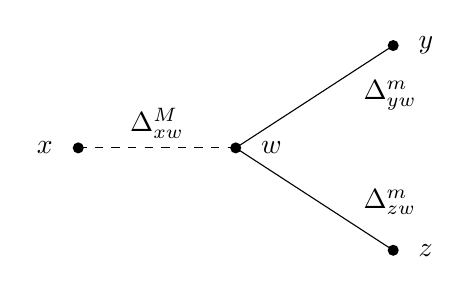
\begin{tikzpicture}[baseline=(current bounding box.center)]
                \begin{feynman}
                  % Vertex with a label
                  % External legs
                  
                  \vertex[label={[shift={(0.2cm, 0cm)}]right:$w$}] (v) at (0, 0);
                  \vertex[label={[shift={(-0.2cm, 0cm)}]left:$x$}]  (a) at (-2, 0);
                  \vertex[label={[shift={(0.2cm, 0cm)}]right:$y$}]  (b) at (2, 1.3);
                  \vertex[label={[shift={(0.2cm, 0cm)}]right:$z$}]  (c) at (2, -1.3);


                  \fill (v) circle (2pt);
                  \fill (a) circle (2pt);
                  \fill (b) circle (2pt);
                  \fill (c) circle (2pt);

                  
                  % Dashed line
                  \diagram* {
                    (a) -- [dashed, edge label={$\Delta_{xw}^{M}$}] (v) [dot],
                    (v) -- [edge label'={$\Delta_{yw}^{m}$}, near end] (b),
                    (v) -- [edge label={$\Delta_{zw}^{m}$}, near end] (c),
                  };
                \end{feynman}
            \end{tikzpicture}
            $B = -ig\int \text{d}^4 w \Delta^M(x-w) \Delta^m(w-y) \Delta^m(w-z)$
            \end{center}
    \end{minipage}\\[0.4cm]
    Where the symmetry factor for the left diagram gains a factor of $2$ from exchanging the endpoints of the internal loop. We have the amplitude 
    \begin{align*}
        G(x, y, z) =  -ig\int \text{d}^4 w \Delta^M(x-w) \Delta^m(w-y) \Delta^m(w-z) -\frac{ig}{2}\int \text{d}^4 w \Delta^M(x-w) \Delta^m(w-w) \Delta^m(y-z) + O(g^2).
    \end{align*}

\newpage
    \item[(c)]
    \begin{enumerate}
        \item[i.] The Fourier transform of the previously computed $A,B$ contribution to the position-space n-point function is 
        \footnotesize{
        \begin{align*}
            \tilde{G}_A(p_1, p_2, p_3) &= -ig\dfrac{1}{2(2\pi)^{4 \times 3}}\int [\cdots] \int  \text{d}^4k_1\text{d}^4k_2\text{d}^4k_3 \int \text{d}^4 w \dfrac{i e^{i k_1(w-w)}}{k_1^2 - m^2 +i\epsilon} \dfrac{i e^{i k_2(x-w)}}{k_2^2 - M^2 +i\epsilon} \dfrac{i e^{i k_3(y-z)}}{k_3^2 - m^2 +i\epsilon}\\
            &= -ig\dfrac{i^3}{2(2\pi)^{4 \times 3}}\int [\cdots]\int \text{d}^4k_1\text{d}^4k_2\text{d}^4k_3 \dfrac{1}{k_1^2 - m^2 +i\epsilon} \dfrac{e^{i k_2(x)}}{k_2^2 - M^2 +i\epsilon}\dfrac{e^{i k_3(y-z)}}{k_3^2 - m^2 +i\epsilon}\int \text{d}^4 w \ e^{i k_2(-w)}\\
            &= -ig\dfrac{i^3}{2(2\pi)^{4 \times 3}}\int [\cdots]\int \text{d}^4k_1\text{d}^4k_2\text{d}^4k_3 \dfrac{1}{k_1^2 - m^2 +i\epsilon} \dfrac{e^{i k_2(x)}}{k_2^2 - M^2 +i\epsilon}\dfrac{e^{i k_3(y-z)}}{k_3^2 - m^2 +i\epsilon} (2\pi)^4 \delta(k_2)\\
            &= -ig\dfrac{i^3}{- M^2 + i \epsilon}\dfrac{1}{2(2\pi)^{4 \times 3}}\int \text{d}^4k_1\text{d}^4k_3 \text{d}^4 y \text{d}^4 z \dfrac{(2\pi)^4\delta(p_1)}{k_1^2 - m^2 +i\epsilon} \dfrac{e^{i (k_3+p_2)y+i(-k_3+p_3)z}}{k_3^2 - m^2 +i\epsilon} (2\pi)^4\\
            &= -ig\dfrac{i^3}{- M^2 + i \epsilon}\dfrac{1}{2(2\pi)^{4 \times 3}}\int \text{d}^4k_1\text{d}^4k_3 \text{d}^4k_1 \dfrac{(2\pi)^4\delta(p_1)}{k_1^2 - m^2 +i\epsilon} \dfrac{(2\pi)^{4 \times 2}\delta^{(4)}(k_3+p_2)\delta^{(4)}(-k_3+p_3)}{k_3^2 - m^2 +i\epsilon} (2\pi)^4\\
            &=-i\dfrac{g}{2}\dfrac{i}{\textcolor{blue}{p_1^2}- M^2 + i \epsilon} \dfrac{i}{p_3^2 - m^2 +i\epsilon}  \dfrac{i}{(2\pi)^4}\int \text{d}^4 k_1 \dfrac{1}{k_1^2 - m^2 +i\epsilon} \times (2\pi)^4 \delta(\textcolor{blue}{p_1})\delta(p_2 + p_3),\\
            \tilde{G}_B(p_1, p_2, p_3) &= -ig\dfrac{1}{(2\pi)^{4 \times 3}}\int [\cdots]\int \text{d}^4k_1\text{d}^4k_2\text{d}^4k_3 \int \text{d}^4 w \dfrac{ie^{i k_1(x-w)}}{k_1^2 - M^2 +i\epsilon} \dfrac{ie^{i k_2(w-y)}}{k_2^2 - m^2 +i\epsilon} \dfrac{ie^{i k_3(w-z)}}{k_3^2 - m^2 +i\epsilon}\\
            &= -ig\dfrac{i^3}{(2\pi)^{4 \times 3}}\int [\cdots]\int \text{d}^4k_1\text{d}^4k_2\text{d}^4k_3 \ \dfrac{e^{i k_1(x)}}{k_1^2 - M^2 +i\epsilon} \dfrac{e^{i k_2(-y)}}{k_2^2 - m^2 +i\epsilon} \dfrac{e^{i k_3(-z)}}{k_3^2 - m^2 +i\epsilon}\times (2\pi)^4 \ \delta^{(4)}(k_2 + k_3 - k_1)\\
            &= -ig\dfrac{i^3}{(2\pi)^{4 \times 3}}\int \text{d}^4k_1\text{d}^4k_2\text{d}^4k_3 \ \dfrac{(2\pi)^4\delta^{(4)}(p_1 + k_1)}{k_1^2 - M^2 +i\epsilon} \dfrac{(2\pi)^4\delta^{(4)}(p_2 - k_2)}{k_2^2 - m^2 +i\epsilon} \dfrac{(2\pi)^4\delta^{(4)}(p_3 - k_3)}{k_3^2 - m^2 +i\epsilon}\times (2\pi)^4 \ \delta^{(4)}(k_2 + k_3 - k_1)\\
            &= -ig \ \dfrac{i}{p_1^2 - M^2 +i\epsilon} \dfrac{i}{p_2^2 - m^2 +i\epsilon} \dfrac{i}{p_3^2 - m^2 +i\epsilon}\times \ (2\pi)^4\delta^{(4)}(p_2 + p_3 + p_1)
        \end{align*}
        }
        where we used the following expression for the (free) Feynman propagator
        \begin{align*}
            \Delta^M(x-x') = \dfrac{1}{(2\pi)^4}\int \text{d}^4k\dfrac{ie^{i k(x-x')}}{k^2 - M^2 +i\epsilon}\quad \& \quad \Delta^m(x-x') = \dfrac{1}{(2\pi)^4}\int \text{d}^4k\dfrac{i e^{i k(x-x')}}{k^2 - m^2 +i\epsilon}
        \end{align*}
        and $\int [\cdots] = \int \text{d}^4x \text{d}^4y \text{d}^4z \ e^{i(p_1 x +p_2 y + p_3 z)}$.
        \item[ii.] We now consider the momentum-space Feynman rules computing the scattering matrix element associated to the $O(g)$ amputated diagrams of item (b).\\[0.5cm]
        \footnotesize{
        \begin{minipage}{0.45\textwidth}
            \begin{center}
                \begin{tikzpicture}[baseline=(current bounding box.center)]
                    \begin{feynman}
                        % Vertex with a label
                        % External legs
                        \vertex [left=of v] (a);
                        \vertex [right=of v] (l);
                        %\vertex [below=1cm of v] (c);
                        \vertex [below=1cm of l] (c);  
                        \vertex [below=1cm of a] (d); % Adjust the vertical position here

                        \vertex (V) at (-1.6 * 0.2 , 0.2) {};
                        \vertex (A) at (-1.6 * 0.8 , 0.2) {};
                        \vertex (V2) at (-0.6-1, -0.2-1) {};
                        \vertex (A2) at (0.6-1, -0.2-1) {};

                        \vertex (V22) at (-0.6+1, -0.2-1) {};
                        \vertex (A22) at (0.6+1, -0.2-1) {};

                        \draw [->] (A) -- (V) node [midway, label=above:$p_1$] {};
                        \draw [->] (V2) -- (A2) node [midway, label=below:$p_3$] {};
                        \draw [->] (A22) -- (V22) node [midway, label=below:$p_2$] {};

                        \fill (a) circle (2pt);
                        \fill (v) circle (2pt);
                        \fill (d) circle (2pt);
                        \fill (c) circle (2pt);

                        \draw[->] (1.4, -0.65) arc (-90:90:0.65cm) node [midway, label=right:$k$] {};
                        
                
                        % Dashed line
                        \diagram* {
                          (a) -- [dashed] (v) -- [half left] (l) -- [half left] (v),
                          (c) -- (d) ,
                        };
                      \end{feynman}
                  \end{tikzpicture} \\[0.3cm]
                  $A$
                \end{center}
                
        \end{minipage}
        %
        \begin{minipage}{0.45\textwidth}
            \vspace{-0.3cm}
            \begin{center}
                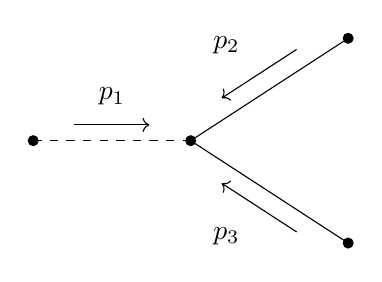
\begin{tikzpicture}[baseline=(current bounding box.center)]
                    \begin{feynman}
                      % Vertex with a label
                      % External legs
                      
                      \vertex (v) at (0, 0);
                      \vertex (a) at (-2, 0);
                      \vertex (b) at (2, 1.3);
                      \vertex (c) at (2, -1.3);
                      \vertex (V) at (-2 * 0.2 , 0.2) {};
                      \vertex (A) at (-2 * 0.8 , 0.2) {};

                      \vertex (V2) at (2 * 0.2 - 1.3 * 0.1, 1.3 * 0.2 + 2 * 0.1) {};
                      \vertex (B) at (2 * 0.8 - 1.3 * 0.1, 1.3 * 0.8 + 2 * 0.1) {};

                      \vertex (V3) at (2 * 0.2 - 1.3 * 0.1, -1.3 * 0.2 - 2 * 0.1) {};
                      \vertex (C) at (2 * 0.8 - 1.3 * 0.1, -1.3 * 0.8 - 2 * 0.1) {};
                      
                      
                      \draw [->] (A) -- (V) node [midway, label=above:$p_1$] {};
                      \draw [->] (B) -- (V2) node [midway, label=above left:$p_2$] {};
                      \draw [->] (C) -- (V3)node [midway, label=below left:$p_3$] {};
                      %\draw [->] (C) -- (V3);
    
                      \fill (v) circle (2pt);
                      \fill (a) circle (2pt);
                      \fill (b) circle (2pt);
                      \fill (c) circle (2pt);
    
                      
                      % Dashed line
                      \diagram* {
                        (a) -- [dashed] (v) [dot],
                        (v) -- [near end] (b),
                        (v) -- [near end] (c),
                      };
                    \end{feynman}
                \end{tikzpicture}\\[0.4cm]            
                $B$
                \end{center}
        \end{minipage}\\[0.4cm]
        }
        $$A = -i\dfrac{g}{2} \ \dfrac{1}{(2\pi)^4}\int \text{d}k^2 \dfrac{i}{k^2 - m^2 +i\epsilon} \times \textcolor{blue}{(2\pi)^4\delta^{(4)}(p_1)} \times \textcolor{red}{(2\pi)^4\delta^{(4)}(p_2+p_3)}$$ where the blue contribution ensures total momentum conservation of the upper diagram and red contribuation ensures total momentum conservation of the lower sub diagram.
        $$B = -ig \times \ \textcolor{blue}{(2\pi)^4\delta^{(4)}(p_2 + p_3 + p_1)}$$
        where the blue contribution ensures the momentum conservation of the entire diagram.
        
        We see that the momentum space Feynman rules for these diagrams produce expression that differ from the Fourier transform of the n-point function at $O(g)$ calculated above. The difference is that the external legs free propagators do not show up in the momentum-space Feynman rules. This is due to the cancelation of these propagators by the interacting mass Klein-Gordon operators of the LSZ formula. More precisely, the momentum-space Feynman rules compute the scattering amplitude for the partially summed n-point function diagrams with all possible bubbles on external legs dressing them so that they get canceled by the Klein-Gordon operators. 
      \end{enumerate}
    \newpage
    \item[(d)] We now suppose that the $\Phi$ field as at least twice as massive as the $\varphi$ field. we are interested in the decay of a $\Phi$ particle with momentum $\mathbf{p}$ to a pair of $\varphi$ particles with 3-momentum $\mathbf{k}_1$ and $\mathbf{k}_2$ (respectively associated to four momenta $p, k_1, k_2$). To compute this scattering amplitude up to next to leading order in $g$, we use the LSZ reduction formula. The formula will involve 3-point functions $\bra{\Omega}T\Phi(x)\varphi(y)\varphi(z)\ket{\Omega}$ like the one treated in items (b) and (c). Since the interaction term of the Lagrangian density has a odd number of operators in it only $g^{\text{odd}}$ terms will appear in the n-point function expansion and scattering amplitude. This means that the leading order contribution is $O(g)$ and the next non-vanishing contribution is $O(g^3)$. The diagrams that contributes to the \textit{decay} amplitude at $O(g^3)$ (only remaining fully connected diagram after amputation) are the following: 
    \begin{equation*}
      \begin{tikzpicture}[baseline=-\the\dimexpr\fontdimen22\textfont2\relax]
        \begin{feynman}
          % External legs
          \vertex[label={left:$\mathbf{p}$}] (a) at (-1, 0);
          \vertex[label={below right:$\mathbf{k}_1$}] (b) at (1, -1);
          \vertex[label={above right:$\mathbf{k}_2$}] (c) at (1, 1);
          



          \fill (a) circle (2pt);
          \fill (b) circle (2pt);
          \fill (c) circle (2pt);
    
          \diagram* {
            (a) -- [dashed] (v),
            (v) -- (b),
            (v) -- (c),
            
          };
        \end{feynman}
      \end{tikzpicture}
      +
      \begin{tikzpicture}[baseline=-\the\dimexpr\fontdimen22\textfont2\relax]
        \begin{feynman}
          % External legs
          \vertex[label={left:$\mathbf{p}$}] (a) at (-1, 0);
          \vertex[label={below right:$\mathbf{k}_1$}] (b) at (1, -1);
          \vertex[label={above right:$\mathbf{k}_2$}] (c) at (1, 1);
          

          \vertex (e) at (0.5, -0.5);
          \vertex (f) at (0.5, 0.5);

          \fill (a) circle (2pt);
          \fill (b) circle (2pt);
          \fill (c) circle (2pt);
          \fill (e) circle (2pt);
          \fill (f) circle (2pt);
    
          \diagram* {
            (a) -- [dashed] (v),
            (v) -- (c),
            (v) -- (e),
            (e) -- [dashed] (f);
            (v) -- (b),
          };
        \end{feynman}
      \end{tikzpicture}
    \end{equation*}
    which maps to the scattering amplitude
    \begin{align*}
      S(\mathbf{p} \to \mathbf{k}_1, \mathbf{k}_2) = \left(-i g  + (-ig)^3 \dfrac{1}{(2\pi)^4} \int \mathbf{d}^4 k \dfrac{i}{k^2 - M^2 + i\epsilon} \dfrac{i}{q_1^2 - m^2 + i\epsilon} \dfrac{i}{q_2^2 - m^2 + i\epsilon}\right) \delta^{(4)}(k_2 + k_1 - p)
    \end{align*}
    where we have used the momentum convention: $q_1, k, q_2$ go in a clockwise direction around the internal loop (and $k$ is associated to the $\Phi$ propagator), $p$ is flowing towards the loop and $k_1, k_2$ away from it.  Four-momentum conservation relates $q_1, q_2$ to $p, k_1, k_2$ as follows 
    \begin{align*}
      &p = q_1 - q_2,\quad  k_2 = q_1 - k\quad \& \quad k_1 = -q_2 + k.
    \end{align*}
    and we have 
    \begin{align*}
      S(\mathbf{p} \to \mathbf{k}_1, \mathbf{k}_2) &= \left(-i g  + (-ig)^3 \dfrac{1}{(2\pi)^4} \int \mathbf{d}^4 k \dfrac{i}{k^2 - M^2 + i\epsilon} \dfrac{i}{(k_2 + k)^2 - m^2 + i\epsilon} \dfrac{i}{(-k_1+ k)^2 - m^2 + i\epsilon}\right) \delta^{(4)}(k_2 + k_1 - p).
    \end{align*}
    Since the amputated external lines are associated to free propagators, they describe particles of free mass $M$ and $m$. This allows to write the amplitude in terms of three-momenta of the external particles with: 
    \begin{align*}
      &(-k_1 + k)^2 = k_1^2 + k^2 - (k^0) (k_1)^0 +2\mathbf{k} \cdot \mathbf{k}_1 =  m^2 + k^2 - 2\sqrt{m^2 +\mathbf{k}_1^2} (k^0) +2\mathbf{k} \cdot \mathbf{k}_1\\
      &(k_2 + k)^2 = k_2^2 + k^2 + (k^0) (k_2)^0 -2\mathbf{k} \cdot \mathbf{k}_2 =  m^2 + k^2 + 2\sqrt{m^2 +\mathbf{k}_2^2} (k^0) -2\mathbf{k} \cdot \mathbf{k}_2
    \end{align*}
    where $\mathbf{k}$ is the three-momentum associated to $k$.

    \newpage
    \item[(e)] 
    \begin{enumerate}
      \item[i.] The following diagrams represent contribute at $O(g^2)$ of the free vacuum expectation value 
      \begin{align*}
        \bra{0}\mathrm{~T}\left(-i \frac{g}{2} \int d^4 y \Phi(y) \varphi^2(y)\right)\left(-i \frac{g}{2} \int d^4 z \Phi(z) \varphi^2(z)\right) \varphi\left(x_1\right) \varphi\left(x_2\right) \varphi\left(x_3\right) \varphi\left(x_4\right)\ket{0}. 
      \end{align*}
    % thanks to chat gpt, thiago and sarra for adivces and help counting and drawing the diagrams
    \begin{equation*}
        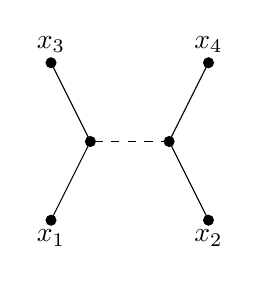
\begin{tikzpicture}[baseline=-\the\dimexpr\fontdimen22\textfont2\relax]
          \begin{feynman}
            % External legs
            \vertex[label={below:$x_1$}] (a) at (-1, -1);
            \vertex[label={below:$x_2$}] (b) at (1, -1);
            \vertex[label={above:$x_3$}] (c) at (-1, 1);
            \vertex[label={above:$x_4$}] (d) at (1, 1);

            \vertex (e) at (-0.5, 0);
            \vertex (f) at (0.5, 0);

            \fill (a) circle (2pt);
            \fill (b) circle (2pt);
            \fill (c) circle (2pt);
            \fill (d) circle (2pt);
            \fill (e) circle (2pt);
            \fill (f) circle (2pt);
      
            \diagram* {
              (a) -- (e),
              (b) -- (f),
              (e) -- (c),
              (f) -- (d),
              (f) -- [dashed] (e),
            };
          \end{feynman}
        \end{tikzpicture}
        +
        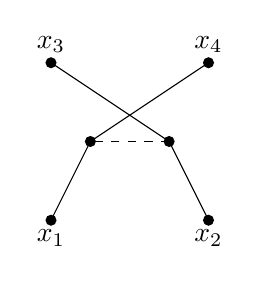
\begin{tikzpicture}[baseline=-\the\dimexpr\fontdimen22\textfont2\relax]
            \begin{feynman}
              % External legs
              \vertex[label={below:$x_1$}] (a) at (-1, -1);
              \vertex[label={below:$x_2$}] (b) at (1, -1);
              \vertex[label={above:$x_3$}] (c) at (-1, 1);
              \vertex[label={above:$x_4$}] (d) at (1, 1);
  
              \vertex (e) at (-0.5, 0);
              \vertex (f) at (0.5, 0);
  
              \fill (a) circle (2pt);
              \fill (b) circle (2pt);
              \fill (c) circle (2pt);
              \fill (d) circle (2pt);
              \fill (e) circle (2pt);
              \fill (f) circle (2pt);
        
              \diagram* {
                (a) -- (e),
                (b) -- (f),
                (e) -- (d),
                (f) -- (c),
                (f) -- [dashed] (e),
              };
            \end{feynman}
          \end{tikzpicture}
          +
          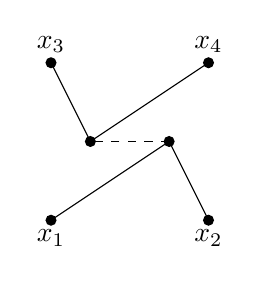
\begin{tikzpicture}[baseline=-\the\dimexpr\fontdimen22\textfont2\relax]
            \begin{feynman}
              % External legs
              \vertex[label={below:$x_1$}] (a) at (-1, -1);
              \vertex[label={below:$x_2$}] (b) at (1, -1);
              \vertex[label={above:$x_3$}] (c) at (-1, 1);
              \vertex[label={above:$x_4$}] (d) at (1, 1);
  
              \vertex (e) at (-0.5, 0);
              \vertex (f) at (0.5, 0);
  
              \fill (a) circle (2pt);
              \fill (b) circle (2pt);
              \fill (c) circle (2pt);
              \fill (d) circle (2pt);
              \fill (e) circle (2pt);
              \fill (f) circle (2pt);
        
              \diagram* {
                (c) -- (e),
                (b) -- (f),
                (e) -- (d),
                (f) -- (a),
                (f) -- [dashed] (e),
              };
            \end{feynman}
          \end{tikzpicture}
    \end{equation*}
    \begin{equation*}
          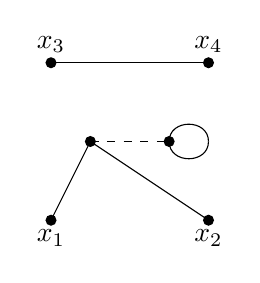
\begin{tikzpicture}[baseline=-\the\dimexpr\fontdimen22\textfont2\relax]
            \begin{feynman}
              % External legs
              \vertex[label={below:$x_1$}] (a) at (-1, -1);
              \vertex[label={below:$x_2$}] (b) at (1, -1);
              \vertex[label={above:$x_3$}] (c) at (-1, 1);
              \vertex[label={above:$x_4$}] (d) at (1, 1);
  
              \vertex (e) at (-0.5, 0);
              \vertex (f) at (0.5, 0);
              \vertex (l) at (1, 0);
  
              \fill (a) circle (2pt);
              \fill (b) circle (2pt);
              \fill (c) circle (2pt);
              \fill (d) circle (2pt);
              \fill (e) circle (2pt);
              \fill (f) circle (2pt);
        
              \diagram* {
                (a) -- (e),
                (b) -- (e),
                (c) -- (d),
                (e) -- [dashed] (f) -- [half left] (l) -- [half left] (f),
              };
            \end{feynman}
          \end{tikzpicture}
          +
          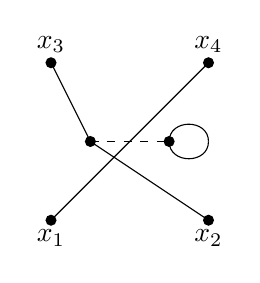
\begin{tikzpicture}[baseline=-\the\dimexpr\fontdimen22\textfont2\relax]
            \begin{feynman}
              % External legs
              \vertex[label={below:$x_1$}] (a) at (-1, -1);
              \vertex[label={below:$x_2$}] (b) at (1, -1);
              \vertex[label={above:$x_3$}] (c) at (-1, 1);
              \vertex[label={above:$x_4$}] (d) at (1, 1);
  
              \vertex (e) at (-0.5, 0);
              \vertex (f) at (0.5, 0);
              \vertex (l) at (1, 0);
  
              \fill (a) circle (2pt);
              \fill (b) circle (2pt);
              \fill (c) circle (2pt);
              \fill (d) circle (2pt);
              \fill (e) circle (2pt);
              \fill (f) circle (2pt);
        
              \diagram* {
                (c) -- (e),
                (b) -- (e),
                (a) -- (d),
                (e) -- [dashed] (f) -- [half left] (l) -- [half left] (f),
              };
            \end{feynman}
          \end{tikzpicture}
          +
          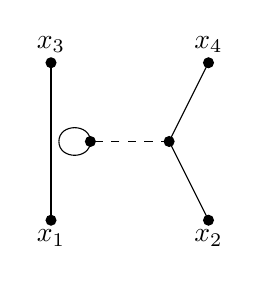
\begin{tikzpicture}[baseline=-\the\dimexpr\fontdimen22\textfont2\relax]
            \begin{feynman}
              % External legs
              \vertex[label={below:$x_1$}] (a) at (-1, -1);
              \vertex[label={below:$x_2$}] (b) at (1, -1);
              \vertex[label={above:$x_3$}] (c) at (-1, 1);
              \vertex[label={above:$x_4$}] (d) at (1, 1);
  
              \vertex (e) at (-0.5, 0);
              \vertex (f) at (0.5, 0);
              \vertex (l) at (-0.9, 0);
  
              \fill (a) circle (2pt);
              \fill (b) circle (2pt);
              \fill (c) circle (2pt);
              \fill (d) circle (2pt);
              \fill (e) circle (2pt);
              \fill (f) circle (2pt);
        
              \diagram* {
                (d) -- (f),
                (a) -- (c),
                (b) -- (f),
                (f) -- [dashed] (e) -- [half left] (l) -- [half left] (e),
              };
            \end{feynman}
          \end{tikzpicture}
          +
          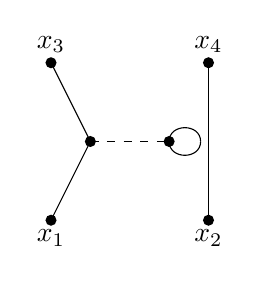
\begin{tikzpicture}[baseline=-\the\dimexpr\fontdimen22\textfont2\relax]
            \begin{feynman}
              % External legs
              \vertex[label={below:$x_1$}] (a) at (-1, -1);
              \vertex[label={below:$x_2$}] (b) at (1, -1);
              \vertex[label={above:$x_3$}] (c) at (-1, 1);
              \vertex[label={above:$x_4$}] (d) at (1, 1);
  
              \vertex (e) at (-0.5, 0);
              \vertex (f) at (0.5, 0);
              \vertex (l) at (0.9, 0);
  
              \fill (a) circle (2pt);
              \fill (b) circle (2pt);
              \fill (c) circle (2pt);
              \fill (d) circle (2pt);
              \fill (e) circle (2pt);
              \fill (f) circle (2pt);
        
              \diagram* {
                (c) -- (e),
                (b) -- (d),
                (a) -- (e),
                (e) -- [dashed] (f) -- [half left] (l) -- [half left] (f),
              };
            \end{feynman}
          \end{tikzpicture}
          +
          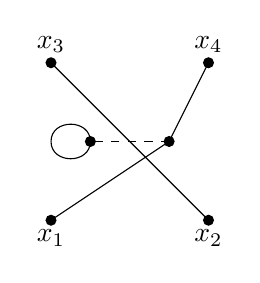
\begin{tikzpicture}[baseline=-\the\dimexpr\fontdimen22\textfont2\relax]
            \begin{feynman}
              % External legs
              \vertex[label={below:$x_1$}] (a) at (-1, -1);
              \vertex[label={below:$x_2$}] (b) at (1, -1);
              \vertex[label={above:$x_3$}] (c) at (-1, 1);
              \vertex[label={above:$x_4$}] (d) at (1, 1);
  
              \vertex (e) at (-0.5, 0);
              \vertex (f) at (0.5, 0);
              \vertex (l) at (-1, 0);
  
              \fill (a) circle (2pt);
              \fill (b) circle (2pt);
              \fill (c) circle (2pt);
              \fill (d) circle (2pt);
              \fill (e) circle (2pt);
              \fill (f) circle (2pt);
        
              \diagram* {
                (d) -- (f),
                (a) -- (f),
                (b) -- (c),
                (f) -- [dashed] (e) -- [half left] (l) -- [half left] (e),
              };
            \end{feynman}
          \end{tikzpicture}
          +
          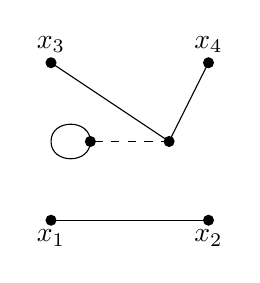
\begin{tikzpicture}[baseline=-\the\dimexpr\fontdimen22\textfont2\relax]
            \begin{feynman}
              % External legs
              \vertex[label={below:$x_1$}] (a) at (-1, -1);
              \vertex[label={below:$x_2$}] (b) at (1, -1);
              \vertex[label={above:$x_3$}] (c) at (-1, 1);
              \vertex[label={above:$x_4$}] (d) at (1, 1);
  
              \vertex (e) at (-0.5, 0);
              \vertex (f) at (0.5, 0);
              \vertex (l) at (-1, 0);
  
              \fill (a) circle (2pt);
              \fill (b) circle (2pt);
              \fill (c) circle (2pt);
              \fill (d) circle (2pt);
              \fill (e) circle (2pt);
              \fill (f) circle (2pt);
        
              \diagram* {
                (a) -- (b),
                (c) -- (f),
                (d) -- (f),
                (f) -- [dashed] (e) -- [half left] (l) -- [half left] (e),
              };
            \end{feynman}
          \end{tikzpicture}
    \end{equation*}
    \begin{equation*}
        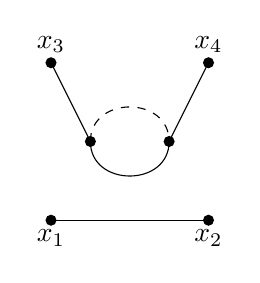
\begin{tikzpicture}[baseline=-\the\dimexpr\fontdimen22\textfont2\relax]
            \begin{feynman}
              % External legs
              \vertex[label={below:$x_1$}] (a) at (-1, -1);
              \vertex[label={below:$x_2$}] (b) at (1, -1);
              \vertex[label={above:$x_3$}] (c) at (-1, 1);
              \vertex[label={above:$x_4$}] (d) at (1, 1);
  
              \vertex (e) at (-0.5, 0);
              \vertex (f) at (0.5, 0);
              \vertex (l) at (0.9, 0);
  
              \fill (a) circle (2pt);
              \fill (b) circle (2pt);
              \fill (c) circle (2pt);
              \fill (d) circle (2pt);
              \fill (e) circle (2pt);
              \fill (f) circle (2pt);
        
              \diagram* {
                (b) -- (a),
                (c) -- (e),
                (e) -- [dashed, half left] (f) -- [half left] (e),
                (f) -- (d),
              };
            \end{feynman}
          \end{tikzpicture}
          +
        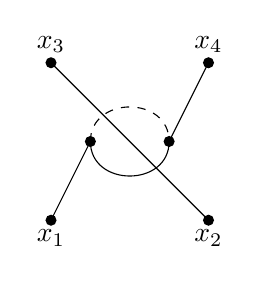
\begin{tikzpicture}[baseline=-\the\dimexpr\fontdimen22\textfont2\relax]
            \begin{feynman}
              % External legs
              \vertex[label={below:$x_1$}] (a) at (-1, -1);
              \vertex[label={below:$x_2$}] (b) at (1, -1);
              \vertex[label={above:$x_3$}] (c) at (-1, 1);
              \vertex[label={above:$x_4$}] (d) at (1, 1);
  
              \vertex (e) at (-0.5, 0);
              \vertex (f) at (0.5, 0);
              \vertex (l) at (0.9, 0);
  
              \fill (a) circle (2pt);
              \fill (b) circle (2pt);
              \fill (c) circle (2pt);
              \fill (d) circle (2pt);
              \fill (e) circle (2pt);
              \fill (f) circle (2pt);
        
              \diagram* {
                (b) -- (c),
                (a) -- (e),
                (e) -- [dashed, half left] (f) -- [half left] (e),
                (f) -- (d),
              };
            \end{feynman}
        \end{tikzpicture}
        + 
        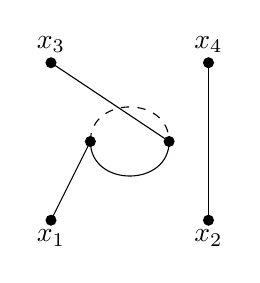
\begin{tikzpicture}[baseline=-\the\dimexpr\fontdimen22\textfont2\relax]
            \begin{feynman}
              % External legs
              \vertex[label={below:$x_1$}] (a) at (-1, -1);
              \vertex[label={below:$x_2$}] (b) at (1, -1);
              \vertex[label={above:$x_3$}] (c) at (-1, 1);
              \vertex[label={above:$x_4$}] (d) at (1, 1);
  
              \vertex (e) at (-0.5, 0);
              \vertex (f) at (0.5, 0);
              \vertex (l) at (0.9, 0);
  
              \fill (a) circle (2pt);
              \fill (b) circle (2pt);
              \fill (c) circle (2pt);
              \fill (d) circle (2pt);
              \fill (e) circle (2pt);
              \fill (f) circle (2pt);
        
              \diagram* {
                (b) -- (d),
                (a) -- (e),
                (e) -- [dashed, half left] (f) -- [half left] (e),
                (f) -- (c),
              };
            \end{feynman}
          \end{tikzpicture}
          +
          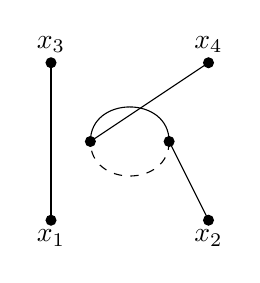
\begin{tikzpicture}[baseline=-\the\dimexpr\fontdimen22\textfont2\relax]
            \begin{feynman}
              % External legs
              \vertex[label={below:$x_1$}] (a) at (-1, -1);
              \vertex[label={below:$x_2$}] (b) at (1, -1);
              \vertex[label={above:$x_3$}] (c) at (-1, 1);
              \vertex[label={above:$x_4$}] (d) at (1, 1);
  
              \vertex (e) at (-0.5, 0);
              \vertex (f) at (0.5, 0);
              \vertex (l) at (0.9, 0);
  
              \fill (a) circle (2pt);
              \fill (b) circle (2pt);
              \fill (c) circle (2pt);
              \fill (d) circle (2pt);
              \fill (e) circle (2pt);
              \fill (f) circle (2pt);
        
              \diagram* {
                (a) -- (c),
                (b) -- (f),
                (f) -- [dashed, half left] (e) -- [half left] (f),
                (e) -- (d),
              };
            \end{feynman}
          \end{tikzpicture}
          +
          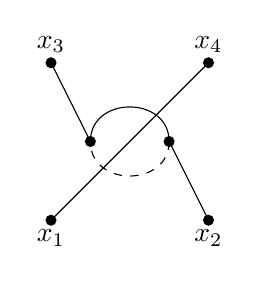
\begin{tikzpicture}[baseline=-\the\dimexpr\fontdimen22\textfont2\relax]
            \begin{feynman}
              % External legs
              \vertex[label={below:$x_1$}] (a) at (-1, -1);
              \vertex[label={below:$x_2$}] (b) at (1, -1);
              \vertex[label={above:$x_3$}] (c) at (-1, 1);
              \vertex[label={above:$x_4$}] (d) at (1, 1);
  
              \vertex (e) at (-0.5, 0);
              \vertex (f) at (0.5, 0);
              \vertex (l) at (0.9, 0);
  
              \fill (a) circle (2pt);
              \fill (b) circle (2pt);
              \fill (c) circle (2pt);
              \fill (d) circle (2pt);
              \fill (e) circle (2pt);
              \fill (f) circle (2pt);
        
              \diagram* {
                (a) -- (d),
                (b) -- (f),
                (f) -- [dashed, half left] (e) -- [half left] (f),
                (e) -- (c),
              };
            \end{feynman}
          \end{tikzpicture}
          +
          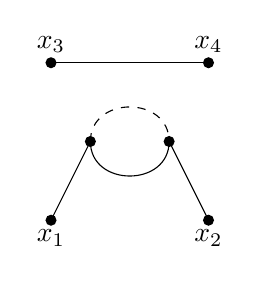
\begin{tikzpicture}[baseline=-\the\dimexpr\fontdimen22\textfont2\relax]
            \begin{feynman}
              % External legs
              \vertex[label={below:$x_1$}] (a) at (-1, -1);
              \vertex[label={below:$x_2$}] (b) at (1, -1);
              \vertex[label={above:$x_3$}] (c) at (-1, 1);
              \vertex[label={above:$x_4$}] (d) at (1, 1);
  
              \vertex (e) at (-0.5, 0);
              \vertex (f) at (0.5, 0);
              \vertex (l) at (0.9, 0);
  
              \fill (a) circle (2pt);
              \fill (b) circle (2pt);
              \fill (c) circle (2pt);
              \fill (d) circle (2pt);
              \fill (e) circle (2pt);
              \fill (f) circle (2pt);
        
              \diagram* {
                (d) -- (c),
                (a) -- (e),
                (e) -- [dashed, half left] (f) -- [half left] (e),
                (f) -- (b),
              };
            \end{feynman}
          \end{tikzpicture}
    \end{equation*}
    \begin{equation*}
        \left[
        \begin{tikzpicture}[baseline=-\the\dimexpr\fontdimen22\textfont2\relax]
            \begin{feynman}
              % External legs
              \vertex[label={below:$x_1$}] (a) at (-1, -1);
              \vertex[label={below:$x_2$}] (b) at (1, -1);
              \vertex[label={above:$x_3$}] (c) at (-1, 1);
              \vertex[label={above:$x_4$}] (d) at (1, 1);
  
              
  
              \fill (a) circle (2pt);
              \fill (b) circle (2pt);
              \fill (c) circle (2pt);
              \fill (d) circle (2pt);
        
              \diagram* {
                (d) -- (c),
                (a) -- (b),
              };
            \end{feynman}
          \end{tikzpicture}
          +
          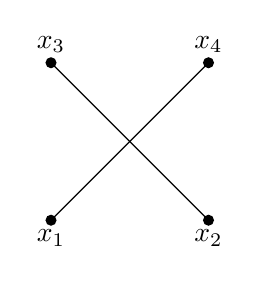
\begin{tikzpicture}[baseline=-\the\dimexpr\fontdimen22\textfont2\relax]
            \begin{feynman}
              % External legs
              \vertex[label={below:$x_1$}] (a) at (-1, -1);
              \vertex[label={below:$x_2$}] (b) at (1, -1);
              \vertex[label={above:$x_3$}] (c) at (-1, 1);
              \vertex[label={above:$x_4$}] (d) at (1, 1);
  
              
  
              \fill (a) circle (2pt);
              \fill (b) circle (2pt);
              \fill (c) circle (2pt);
              \fill (d) circle (2pt);
        
              \diagram* {
                (d) -- (a),
                (b) -- (c),
              };
            \end{feynman}
          \end{tikzpicture}
          +
          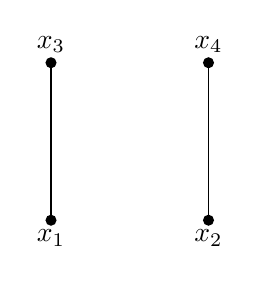
\begin{tikzpicture}[baseline=-\the\dimexpr\fontdimen22\textfont2\relax]
            \begin{feynman}
              % External legs
              \vertex[label={below:$x_1$}] (a) at (-1, -1);
              \vertex[label={below:$x_2$}] (b) at (1, -1);
              \vertex[label={above:$x_3$}] (c) at (-1, 1);
              \vertex[label={above:$x_4$}] (d) at (1, 1);
  
              
  
              \fill (a) circle (2pt);
              \fill (b) circle (2pt);
              \fill (c) circle (2pt);
              \fill (d) circle (2pt);
        
              \diagram* {
                (d) -- (b),
                (a) -- (c),
              };
            \end{feynman}
          \end{tikzpicture}
        \right]
        \times 
        \left[
        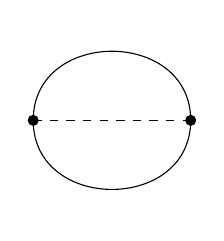
\begin{tikzpicture}[baseline=-\the\dimexpr\fontdimen22\textfont2\relax]
            \begin{feynman}
              % External legs
              \vertex (a) at (-1, 0);
              \vertex (b) at (1, 0);
  
              \fill (a) circle (2pt);
              \fill (b) circle (2pt);
        
              \diagram* {
                (a) -- [half left] (b) -- [half left] (a),
                (a) -- [dashed] (b),
              };
            \end{feynman}
          \end{tikzpicture}
          +
          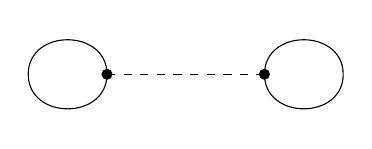
\begin{tikzpicture}[baseline=-\the\dimexpr\fontdimen22\textfont2\relax]
            \begin{feynman}
              % External legs
              \vertex (a) at (-1, 0);
              \vertex (b) at (1, 0);
              \vertex (l1) at (2, 0);
              \vertex (l2) at (-2, 0);
  
              \fill (a) circle (2pt);
              \fill (b) circle (2pt);
        
              \diagram* {
                (a) -- [half left] (l2) -- [half left] (a),
                (b) -- [half left] (l1) -- [half left] (b),
                (a) -- [dashed] (b),
              };
            \end{feynman}
          \end{tikzpicture}
        \right]
    \end{equation*}
    \item[ii.] The subset of diagrams in i. that contributes to the four-point function 
    \begin{align*}
    G\left(x_1, x_2, x_3, x_4\right)=\bra{\Omega}\mathrm{T} \varphi\left(x_1\right) \varphi\left(x_2\right) \varphi\left(x_3\right) \varphi\left(x_4\right)\ket{\Omega}
    \end{align*}
    at order $g^2$ is given by the three first row since the normalisation factor arising for the expression of $\ket{\Omega}$ in terms of $\ket{0}$ cancels all diagrams with vacuum subdiagrams (in the right bracket). 
    \item[iii.] The subset of diagrams that contributes to the $\varphi \varphi \rightarrow \varphi \varphi$ matrix element $i \mathcal{M}\left(\varphi\left(\mathbf{k}_1\right) \varphi\left(\mathbf{k}_2\right) \rightarrow \varphi\left(\mathbf{p}_1\right) \varphi\left(\mathbf{p}_2\right)\right)$ at $O(g^2)$ is given by the first row since it contains the only diagrams that persist after amputation and removal of diagrams with vacuum subdiagrams. Indeed the second and thirs rows are mapped to free propagation by amputation and do not contribute to $O(g)$.  
  \end{enumerate}
  \item[(f)] In item (e) i. and ii. are related trough the relation between the free vacuum n-point function (has vacuum subdiagrams) and the interacting vaccuum n-point functions (has its vacuum subdiagram contributions canceled by the normalisation). Item (e) ii. and iii. are related trough the LSZ formula that leads to amputation of the bubbles on the external lines of the diagrams that contribute to the n-point functions of the interacting vacuum. 
  \newpage
  \item[(g)] The second row first diagram of item (e) i. has a symmetry factor of $2$ because the internal loop end points can be exchanged while keeping the end point fixed and this operation is the only such symmetry of the diagram. Wicks theoreme can be used to recover the same symmetry factor from Wick contractions in the free vacuum n-point function apearing in the perturbative expansion of the LSZ reduction formula. Ignoring the normalisation of the vacuum (because our analysed diagram contains no vacuum subdiagrams), we start from the following free vacuum n-point function
  \begin{align*}
    \dfrac{(-ig)^2}{\textcolor{red}{2!}\textcolor{blue}{(2!1!)^2}}\bra{0}T \varphi(x_1)\varphi(x_2)\varphi(x_3)\varphi(x_4)\Phi(y) \varphi(y)\varphi(y)\Phi(x) \varphi(x)\varphi(x) \ket{0}
  \end{align*}
  where the blue factor comes from the Lagrangian density and the red one from the taylor expansion in powers of $g$. The blue factor is associated to the number of fields connecting to a vertex and the red one is associated to the number of verticies. Wick's theorem allows to write this n-point function as the sum of all fully contracted wick operators. Each wick contraction of same type fields corresponds to a Feynman diagram edge between the contracted points where the contracted fields are evaluated. In our case the contraction of $\varphi(x_3)$ and $\varphi(x_4)$ necessarely appears because $x_3$ and $x_4$ are joigned and disconnected from the rest of the diagram. The follwong full contractions all map to the same diagram:
  \begin{align*}
    &\wick[below]{\c2\varphi(x_1)\c3\varphi(x_2)\c1\varphi(x_3)\c1\varphi(x_4)\c4\Phi(y) \c2\varphi(y)\c3\varphi(y)\c4\Phi(x) \c2\varphi(x)\c2\varphi(x)}\\[0.3cm]
    &\wick[below]{\c2\varphi(x_1)\c3\varphi(x_2)\c1\varphi(x_3)\c1\varphi(x_4)\c4\Phi(y) \c3\varphi(y)\c2\varphi(y)\c4\Phi(x) \c2\varphi(x)\c2\varphi(x)}\\[0.3cm]
    &\wick[below]{\c5\varphi(x_1)\c2\varphi(x_2)\c1\varphi(x_3)\c1\varphi(x_4)\c3\Phi(y) \c4\varphi(y)\c4\varphi(y)\c3\Phi(x)\c5\varphi(x)\c2\varphi(x)}\\[0.3cm]
    &\wick[below]{\c5\varphi(x_1)\c2\varphi(x_2)\c1\varphi(x_3)\c1\varphi(x_4)\c3\Phi(y) \c4\varphi(y)\c4\varphi(y)\c3\Phi(x)\c2\varphi(x)\c5\varphi(x)}.\\[0.3cm]
  \end{align*}
These $4$ contractions relating to the same diagram, the combinatorial factor in the amplitude becomes 
\begin{align*}
  \dfrac{4}{\textcolor{red}{2!}\textcolor{blue}{(2!1!)^2}} = \dfrac{1}{2} = \dfrac{1}{S}.
\end{align*}
The symmetry factor is linked to the number of wick contractions leading to the same diagram trough the combinatorial factors apearing in the lagrangian density and the perturbative expansion of the LSZ formula. 
\end{enumerate}



\section{Acknowledgement}
Thanks to Thiago and ChatGPT for help drawing the diagrams. Thanks to Thomas for pointing out that amputation reduces the number of relevant $O(g^3)$ digrams to $1$ in item (d).

% References
\makereferences
%-------------------------------------------------------


%%%%%%%%%%%%%%%%%%%%%%%%
% Terminer le document %
%%%%%%%%%%%%%%%%%%%%%%%%
\end{document}